\documentclass[a4paper, 11pt, twoside]{article}  % Based on the ECS Thesis style
\usepackage{graphicx}
\usepackage{makeidx}
% \graphicspath{figures/}  % Location of the graphics files
\usepackage{multirow}
\usepackage{threeparttable}
% Making R code work!
\usepackage{listings}
\usepackage{color}
\usepackage{hyperref}
\usepackage{booktabs}

\hypersetup{urlcolor=blue, colorlinks=false, hypertexnames=true}  % Colours hyperlinks in blue, but this can be distracting 
\usepackage{cleveref}
\definecolor{dkgreen}{rgb}{0,0.6,0}
\definecolor{gray}{rgb}{0.5,0.5,0.5}
\definecolor{mauve}{rgb}{0.58,0,0.82}

\lstset{ %
  language=R,                % the language of the code
   basicstyle=\normalsize\ttfamily,           % the size of the fonts that are used for the code
%   numbers=left,                   % where to put the line-numbers
%   numberstyle=\tiny\color{gray},  % the style that is used for the line-numbers
%   stepnumber=2,                   % the step between two line-numbers. If it's 1, each line
                                  % will be numbered
%   numbersep=5pt,                  % how far the line-numbers are from the code
%   backgroundcolor=\color{white},      % choose the background color. You must add \usepackage{color}
%   showspaces=false,               % show spaces adding particular underscores
%   showstringspaces=false,         % underline spaces within strings
%   showtabs=false,                 % show tabs within strings adding particular underscores
   frame=false,                   % adds a frame around the code
   rulecolor=\color{white},        % if not set, the frame-color may be changed on line-breaks within not-black text (e.g. commens (green here))
%   tabsize=2,                      % sets default tabsize to 2 spaces
%   captionpos=b,                   % sets the caption-position to bottom
%   breaklines=true,                % sets automatic line breaking
%   breakatwhitespace=false,        % sets if automatic breaks should only happen at whitespace
%   title=\lstname,                   % show the filename of files included with \lstinputlisting;
                                  % also try caption instead of title
  keywordstyle=\color{blue},          % keyword style
  commentstyle=\color{dkgreen},       % comment style
  stringstyle=\color{mauve},         % string literal style
  escapeinside={\%*}{*)},            % if you want to add a comment within your code
  morekeywords={*,...}               % if you want to add more keywords to the set
} 

% Include any extra LaTeX packages required
\usepackage[round,]{natbib}  % Use the "Natbib" style for the references
\usepackage{verbatim}  % Needed for the "comment" environment to make LaTeX comments
\usepackage{wallpaper}
\usepackage{cases}
\makeindex
% \renewcommand{\includegraphics}[2][]{\fbox{#2}} %omits images
\begin{document}
 
\title{An introduction to spatial microsimulation with R}
% \author{Robin Lovelace --- R.Lovelace at. Leeds. ac. uk}
\pagestyle{myheadings}
\author{Lovelace, Robin\\
\texttt{r.lovelace@leeds.ac.uk}}
\maketitle

\section{Introduction}

This booklet was written to accompany a two day course of the same title.
As well as providing useful information to the $\approx$30 participants during
and after the course, it is hoped that the material will be of use to others.
Spatial microsimulation is shrouded by an unnecessary mystery, and this is not
helped by the fact that most academic papers on subject and even many textbooks
on the subject are devoid of reproducible examples. In today's age of fast
internet connections, open access datasets and free software, this is an
abomination, damaging to the growth and credibility of the field.

To those doubting the value of this practical approach, I ask the following
questions: If only a small community of researchers hold the majority of the
code needed to perform spatial microsimulation, how can the technique spread
rapidly to other applications? If every PhD student undertaking spatial
microsimulation must start from scratch, how are the methods going to be
refined and improved in a systematic fashion? Most importantly, if the results
of most spatial microsimulation research is not reproducible --- as is currently
the case --- how can we trust them?

This final point is critical not only to spatial microsimulation but the
disciplines of which it is part. Reproducibility is a prerequisite of
falsifiability --- if the method
underlying a result cannot be replicated by others, how can the finding
possibly be falsified? Moreover, the argument continues, any knowledge or
theory can only claim to enter the realm of `science' if it cannot be falsified.
Because it is impossible to prove any proposition in every and all cases, the
only reliable test we can apply is whether or not it can be \emph{disproved}:
falsified via a contradictory finding. This is how scientific progress is made
\citep{Popper1959}. By writing non-reproducible research, researchers may
inadvertently damage the disciplines in which they work. %. how???

Despite and because of these philosophical antecedents, the course is
unashamedly practical. The aim is simple: to provide an accessible yet
deep foundation in spatial microsimulation. This involves both
\emph{understanding} and \emph{implementation} of the technique.
Following the `learning by doing' ethic, the former can best be
attained through the latter: spatial microsimulation need not be an abstract
process that one simply reads about. It can be practical tool used by anyone
with the know-how. As \citet[xxii]{kabacoff2011r} put it regarding R, ``the best
way to learn is to experiment'' and the same applies to spatial microsimulation.

The examples presented below were developed during a PhD project in the energy
costs of commuting. Although some of the code and most of the descriptive text
has been rewritten since then, many of the ideas and methods are described in
more detail in the resulting thesis.% \citep{Lovelace2014-thesis}.

\section{Why R?} \label{setsim} % Move this to just before R implementation?

Software decisions have a major impact on the model's flexibility, efficiency,
reproducibility and
ease of coding. \citet[p.~153]{Holm1987} observed that ``little attention is
paid to the choice of programming language used.''
This appears to be as true now as it was then: software is rarely discussed in
spatial microsimulation papers. 
In my own spatial microsimulation research, a conscious decision was made early
on to use R, with impacts on model features, analysis
and even design. It is thus worth understanding the tool a little before we
begin to use it. The theory is discussed in \cref{s:theory}

% \subsection{Why R?}
The world is awash with computer programming languages and many of these
are general purpose and `Turing complete', meaning they could, with sufficient
effort, perform spatial microsimulation. So why would one chose R?
The most important criteria of evaluation include flexibility,
speed of processing and, most importantly, ease and speed of writing code.
R excels in each of these areas, especially the final one: it
is possible to say a lot in R in few lines of code. Further
are provided by \citet{Matloff-R}:

\begin{itemize}
\item ``a public-domain implementation of the widely-regarded S statistical
language; R/S is the de facto standard among professional statisticians
\item comparable, and often superior, in power to commercial products in most
senses
\item available for Windows, Macs, Linux
\item in addition to enabling statistical operations, it's a general programming
language, so that you can
automate your analyses and create new functions
\item object-oriented and functional programming structure
\item your data sets are saved between sessions, so you don't have to reload
each time
\item open-software nature means it’s easy to get help from the user
community''
\end{itemize}
% Add in disadvantages here.

\section{IPF theory: a worked example} \label{s:theory}
IPF is a simple statistical procedure, ``in which cell counts in a contingency
table containing the sample observations are scaled to be consistent with
various externally given population marginals'' \citep{mcfadden2006testing}. In
other words, and in the context of \emph{spatial} microsimulation, IPF produces
maximum likelihood estimates for the frequency with which people appear in
different areas. The method is also known as `matrix raking' or the RAS
algorithm,
% (\citealp{Lovelace2014-ipf})
and has been described as one
particular instance of a more general procedure of `entropy maximisation'
\citep{Johnston1993}.
The mathematical properties of IPF
are described in earlier papers (e.g.~\citealp{Fienberg1970}).
A practical example of the procedure can be found in
\citet{Norman1999a}, who provides an implementation in Microsoft Excel.

% As \citet{Birkin1988} point out, IPF undertakes the basic task of
% generating a vector of individual characteristics, $x = (x_1, x_2, ..., x_m)$ on the
% basis of a joint probability distribution $p(x)$. Once the probability distribution
% for such a vector is generated, representative
% individuals can be synthesised or extracted from a pre-existing survey dataset.
% However, when information is not available for the full joint distribution, there
% is a need to construct a product of conditional and marginal probabilities,
% by building one attribute at a time, so that the probability of certain attributes
% is conditionally dependent on existing attributes \citep{Birkin1988}:
%
% \begin{equation}
% p(x) = p(x_1)p\left( \frac{x_2}{x_1}\right) p\left( \frac{x_3}{x_2}, x_1\right) \times
%  ... \times p\left( \frac{x_m}{x_{m-1}},...,x_1\right)
% \end{equation}
%
% IPF can be used to model the joint probability distribution
% $p(x_1, x_2, x_3)$ subject to known probabilities
% $p(x_1, x_2)$ and $p(x_1, x_3)$. Following \citet{Birkin1988} and \citet{Ballas2007simb},
% if $p(x_1, x_2, x_3)$ is the $i^{th}$ approximation to the three-attribute joint probability
% vector then:
% \begin{equation}
%  p^1(x_1, x_2, x_3) = \frac{1}{N_1 N_2 N_3}
% \end{equation}
% where $N_j$ is the number of possible states associated with the attribute vector $x$.
% The vector can then be adjusted in \emph{proportion} to the following known constraints:
% \begin{equation}
% p^2(x_1, x_2, x_3) = p^1(x_1, x_2, x_3) \frac{p(x_1, x_2)}
% {{\displaystyle \sum^{}_{x_3}{p^1(x_1, x_2, x_3)}}}
% \label{eq:p2}
% \end{equation}
% \begin{equation}
% p^3(x_1, x_2, x_3) = p^2(x_1, x_2, x_3) \frac{p(x_1, x_3)}
% {{\displaystyle \sum^{}_{x_2}{p^1(x_1, x_2, x_3)}}}
% \label{eq:p3}
% \end{equation}
% IPF involves iterating through equations \ref{eq:p2} and \ref{eq:p3}
% until a \emph{fitted} distribution is obtained, when the probabilities
% are convergent within some acceptable limit \citep{Birkin1988, Fienberg1970, Ballas2007simb}.
% This procedure can be generalised to a larger number of attributes \citep{Birkin1988}:
% if we let $Z_k(x)$ be a subset of the set of attribute vectors
% $E(x)$ for which marginal joint probabilities are known and let $W_k(x)$ be
% the complement of $Z_k(x)$, that is $W_k(x)= E(x) - Z_k(x)$, then:
%
% \begin{equation}
%  p^1(x) = \frac{1}{\displaystyle{\prod^{m}_{i=1}{Ni}}}
% \end{equation}
% \begin{equation}
%  p^2(x) =  p^1(x) \frac{p[Z_1(x)]}{\displaystyle{\sum^{}_{W_1(x)}{p^1(x)}}}
% \label{eq:six}
% \end{equation}
%
% {\centering
% .
%
% .
%
% .
%
% }
%
% \begin{equation}
%  p^{k+1}(x) =  p^k(x) \frac{p[Z_k(x)]}{\displaystyle{\sum^{}_{W_k(x)}{p^k(x)}}}
% \label{eq:seven}
% \end{equation}
%
% IPF iterates through equations \ref{eq:six} and \ref{eq:seven} until convergence
% \citep{Birkin1988}. An extensive discussion of the mathematical properties of
% IPF can be found in \citet{Fienberg1970}.

The simple example below demonstrates how IPF works.
Table \ref{t:w}  describes a
hypothetical microdataset comprising 5 individuals, who are defined by two
constraint variables: age and sex. Each has two categories.
Table \ref{t:s} contains aggregated data
for a hypothetical area. \Cref{t:s2} illustrates this table in a different form,
which shows our ignorance of interaction between age and sex.


\begin{table}[h]
\centering
\caption[A hypothetical input microdata set]{A
hypothetical input microdata set (the original
weights set to one). The bold value is used subsequently for
illustrative purposes.}
\begin{tabular}{llll}
\toprule
{Individual } & {Sex} & {Age-group} & {Weight} \\
\midrule
1 & Male & Over-50 & 1 \\
2 & Male & Over-50 & 1 \\
3 & {Male} & {Under-50} & \textbf{1} \\
4 & Female & Over-50 & 1 \\
5 & Female & Under-50 & 1 \\
\bottomrule
\end{tabular}
\label{t:w}
\end{table}
\vspace{1cm}


\begin{table}[htbp]
\centering
\caption{Hypothetical small area constraints data ($s$).}
\begin{tabular}{cllll}
\toprule
Constraint $\Rightarrow$ & \multicolumn{2}{c}{$i$}& \multicolumn{2}{c}{$j$}\\
Category $\Rightarrow$ & $i_1$ & $i_2$ & $j_1$ & $j_2$ \\
Area $\Downarrow$  & Under-50 & Over-50 &  Male & Female\\
1  & 8 & 4 & 6 & 6\\
\bottomrule
\end{tabular}
\label{t:s}
\end{table}
\vspace{1cm}

\begin{table}[htbp]
\centering
\caption[Small area constraints expressed as marginal totals]{Small
area constraints expressed as marginal totals, and the cell
values to be estimated.}
\begin{tabular}{cllll}\toprule
Marginal totals&  & \multicolumn{2}{c}{$j$} & \\
& Age/sex & Male & Female & T\\ \midrule
\multirow{2}{*}{$i$} & Under-50 & \textbf{?} & ? & 8\\
& Over-50 & ? & ? &4 \\
& T & 6 & 6 &12\\
\bottomrule
\end{tabular}
\label{t:s2}
\end{table}

Table \ref{t:m} presents the
hypothetical microdata in aggregated form,
that can be compared directly to Table \ref{t:s2}.

\begin{table}[htbp]
\centering
\caption[The aggregated results of the weighted
microdata set]{The aggregated results of the weighted
microdata set ($m(1)$).
Note, these values depend on the
weights allocated in Table \ref{t:w} and therefore
 change after each iteration}

\begin{tabular}{cllll}\toprule
Marginal totals&  & \multicolumn{2}{c}{$j$} & \\
& Age/sex & Male & Female & T\\ \midrule
\multirow{2}{*}{$i$} & Under-50 & \textbf{1} & 1 & 2\\
& Over-50 & 2 & 1 &3 \\
& T & 3 & 2 &5\\
\bottomrule
\end{tabular}
\label{t:m}
\end{table}

Using these data it is possible to readjust the weights of the hypothetical
individuals, so that their sum would add up to the totals given in Table
\ref{t:s2} (12). In particular, the weights can be readjusted by multiplying them by
the marginal totals, originally taken from
Table \ref{t:s} and then divided by the respective marginal total in \ref{t:m}.
Because the total for each small-area constraint is 12, this must be
done one constraint at a time. This
can be expressed, for a given area and a given constraint ($i$
or age in this case), as follows:

\begin{equation}
w(n+1)_{ij} = \frac{w(n)_{ij} \times sT_{i}}{mT(n)_{i}}
\label{eq:ipf}
\end{equation}
where $w(n+1)_{ij}$ is the new weight for individuals with characteristics $i$
(age, in this case), and $j$ (sex),  $w(n)_{ij}$ is the original
weight for individuals with these characteristics, $sT_{i}$ is element
marginal total of the small area constraint, $s$
(Table \ref{t:s}) and $mT(n)_{i}$ is the marginal total of category
$j$ of the aggregated results of the weighted
microdata, $m$ (Table \ref{t:m}). $n$ represents the iteration number.
Although the marginal totals of $s$ are known, its cell values
are unknown. Thus, IPF estimates the interaction (or cross-tabulation)
between constraint variables.
(Follow the emboldened values in the tables
to see how the new weight of individual 3 is calculated for the sex constraint.)
Table \ref{t:new-weights} illustrates the weights that result. Notice that the
sum of the weights is equal to the total population, from the constraint variables.

\begin{table}[htbp]
\centering
\caption{Reweighting the hypothetical microdataset in order to fit
Table \ref{t:s}.}
\begin{tabular}{lllll}
\toprule
{Individual} & {Sex} & {age-group} & {Weight} &
{New weight, w(2)} \\ \midrule
1 & Male & Over-50 & 1 & $1 \times 4/3 = \frac{4}{3}$ \\
2 & Male & Over-50 & 1 & $1 \times 4/3 = \frac{4}{3}$ \\
3 & Male & Under-50 & 1 & $\textbf{1} \times
\textbf{8}/\textbf{2} = 4$ \\
4 & Female & Over-50 & 1 & $1 \times 4/3 = \frac{4}{3}$ \\
5 & Female & Under-50 & 1 & $1 \times 8/2 = 4$ \\
\bottomrule
\end{tabular}
\label{t:new-weights}
\end{table}

After the individual level data have been re-aggregated (\cref{t:m2}),
the next stage is to repeat \cref{eq:ipf} for the age constraint to generate a
third set of weights, by replacing
the $i$ in $sT_{i}$ and $mT(n)_{i}$ with $j$ and incrementing the value of n:

\begin{equation}
w(3)_{ij} = \frac{w(2)_{ij} \times sT_{j}}{mT(2)_{j}}
\label{eq:ipf2}
\end{equation}

To test your understanding of IPF, apply \cref{eq:ipf2} to the information above
and that presented in \cref{t:m2}.
This should result in the following vector of new weights, for individuals 1 to
5. Calculate the correct values and pencil them in in place of the question
marks. One `sanity' check of your method here is whether the sum of these
weights is still equal to twelve. % Add online link to answers - tinyurl

\begin{equation}
w(3) = (\frac{6}{5}, \frac{?}{?}, \frac{18}{5}, \frac{?}{?}, \frac{9}{2})
% w(3) = (\frac{6}{5}, \frac{6}{5}, \frac{18}{5}, \frac{3}{2}, \frac{9}{2})
\end{equation}

Notice also that after each iteration the fit between the marginal
totals of $m$ and $s$
improves. The total absolute error (TAE) improves
between $m(1)$ to $m(2)$, falling from
14 to 6 in \cref{t:m} and \cref{t:m2} above. TAE for $m(3)$ (not shown,
but calculated by aggregating $w(3)$) improves even more, to 1.3.
This number would eventually converge to 0 through subsequent
iterations, as there are no empty cells in the input microdataset;
a defining feature of IPF.


\begin{table}[htbp]
\centering
\caption[Aggregated results after constraining for age]{The
aggregated results of the weighted
microdata set after constraining for age ($m(2)$).
}

\begin{tabular}{cllll}\toprule
Marginal totals&  & \multicolumn{2}{c}{$i$} & \\
& Age/sex & Male & Female & T\\ \midrule
\multirow{2}{*}{$j$} & Under-50 & 4 & 4 & 8\\
& Over-50 & $\frac{8}{3}$ & $\frac{4}{3}$ & 4 \\
& T & $6\frac{2}{3}$ & 5$\frac{1}{3}$ & 12\\
\bottomrule
\end{tabular}
\label{t:m2}
\end{table}

The above process, when applied to more categories (e.g. socio-economic class)
and repeated iteratively until a satisfactory convergence occurs, results in a
series of weighted microdatasets, one for each of the small areas being
simulated. This allows for the estimation of variables whose values are not
known at the local level (e.g. income). An issue
with the results of IPF (absent from combinatorial optimisation methods),
however, is that it results in non-integer weights: fractions of individuals
appear in simulated areas. As described in the introduction, this is not ideal
for certain applications. Integer weights allow the results of spatial
microsimulation to be further processed using dynamic microsimulation and agent
based modelling techniques \citep{Pritchard2012}.


% A key benefit from a policy perspective is that
% IPF and other spatial microsimultion techniques
% can provide estimation of variables whose values are not
% known at the local level (e.g. income).
Spatial microsimulation can also provide insight into the likely
distribution of individual level variables about which only
geographically aggregated statistics have been made available.
An issue
with the results of IPF (absent from combinatorial optimisation methods),
however, is that it results in non-integer weights: fractions of individuals
appear in simulated areas.

\section{Implementing IPF in R} \label{simplementing} % priority: automate!!!
The above example is best undertaken by hand, probably with a pen and paper
to gain an understanding of IPF, before the process is automated for 
larger datasets. This section explains how the IPF
algorithm described above was implemented in R, using a slightly more
complex example.
% This section is based on ``Spatial microsimulation in R: a
% beginner’s guide to iterative proportional fitting (IPF)'', a tutorial
% written to accompany a methods paper on integerisation
\citep{Lovelace2013-trs}.\footnote{This tutorial is available from Rpubs, a site dedicated
to publishing R analyses that are reproducible. It uses the RMarkdown
mark-up language, which enables R code to be run and presented within
documents. See http://rpubs.com/RobinLovelace/5089 \label{fnrpub} .}

\emph{Loading in the data}

In the full model the input datasets are stored as .csv files, one for each
constraint and one for the input microdata, and read in with the command
\verb read.csv . For the purposes of understanding how the model works,
the dataset is read line by line, following the
example above. The following code creates example datasets,
based on the same hypothetical survey of 5 individuals described above,
and 5 small areas. The spatial microsimulation model will select individuals
based on age and sex and mode of transport (mode of transport
is also used on the larger online example described in footnote \ref{fnrpub}).
For consistency with the (larger) model used for the paper, 
the individual level data will be referred to as USd (Understanding Society dataset)
and the geographic data as all.msim (for all constraint variables).
The code to read-in the individual level data are presented in code sample \ref{cusd}.
When called, the data are then displayed as a table (see listing \ref{cout}).
\begin{lstlisting}[float=h, caption={Manual input of individual level data
in R}, label=cusd]
# Read in the data in long form (normaly read.table() used)
c.names <- c("id", "age", "sex")
USd <- c(       1, 59, "m",
                2, 54, "m",
                3, 35, "m",
                4, 73, "f",
                5, 49, "f")
USd <- matrix(USd, nrow = 5, byrow = T) # Long data into matrix
USd <- data.frame(USd) # Convert this into a dataframe
names(USd) <- c.names # Add correct column names
USd$age <- as.numeric(levels(USd$age)[USd$age]) # Age is a numeric
\end{lstlisting}
\begin{lstlisting}[float=h, caption={Output of the USd data frame}, label=cout]
USd # Show the data frame in R
##   id age sex
## 1  1  59   m
## 2  2  54   m
## 3  3  35   m
## 4  4  73   f
## 5  5  49   f
\end{lstlisting}
The same procedure applies to the geographical data (listing \ref{cgeo}).
\begin{lstlisting}[float=h*, caption={Geographic data input}, label=cgeo]
 category.labels <- c("16-49", "50+" # Age constraint
             ,"m", "f" # Sex constraint
             # more constraints could go here
             )
all.msim <- c(  8, 4,    6, 6,   # Original aggregate data
                2, 8,    4, 6,   # Elderly
                7, 4,    3, 8,   # Female dominated
                5, 4,    7, 2,   # Male dominated
                7, 3,    6, 4    # Young
                )
all.msim <- matrix(all.msim, nrow = 5, byrow = T) 
all.msim <- data.frame(all.msim) # Convert to dataframe
names(all.msim) <- category.labels # Add correct column names
\end{lstlisting}

IPF relies on the assumption that all constraint variables will contain the
same number of people. This is logical (how can there be more people classified
by age than by sex?) but can cause problems for constraint variables that use
only a subset of the total population, such as those who responded to questions on
travel to work. To overcome this problem, it is possible to normalise the
constraint variables, setting the total for each to the one that has the most
reliable total population. This worked example simply checks whether
or not they are (listing \ref{ccheck}).

\begin{lstlisting}[float=h, caption={R code to check the constrain populations
match}, label=ccheck]
 # Check totals for each constraint match
rowSums(all.msim[,1:2]) # Age constraint
## [1] 12 10 11  9 10
rowSums(all.msim[,3:4]) # Sex constraint
## [1] 12 10 11  9 10

rowSums(all.msim[,1:2]) == rowSums(all.msim[,3:4])
## [1] TRUE TRUE TRUE TRUE TRUE
\end{lstlisting}

\emph{Reweighting the survey dataset}

Iterative proportional fitting determines the weight allocated to each
individual for each zone to best match the geographically aggregated data.
A weight matrix is therefore created, with rows corresponding to individuals
and columns to zones, as described in \cref{s:theory}. In
R, this, and the creation of the aggregated results matrix,
is done with code presented in listing
\ref{cws}).\footnote{In subsequent
versions of the model, single, multi-dimensional weight and
aggregated result matrices are used,
to reduce the length of the scripts.
} 

\begin{lstlisting}[float=h, caption={Creating arrays of weights in R},
label=cws]
weights0 <- array(dim=c(nrow(USd),nrow(all.msim)))
weights1 <- array(dim=c(nrow(USd),nrow(all.msim)))
weights2 <- array(dim=c(nrow(USd),nrow(all.msim)))

weights0[,] <- 1 # sets initial weights to 1

USd.agg <- array(dim=c(nrow(all.msim),ncol(all.msim)))
USd.agg1 <- array(dim=c(nrow(all.msim),ncol(all.msim)))
USd.agg2 <- array(dim=c(nrow(all.msim),ncol(all.msim)))
colnames(USd.agg1) <- category.labels
\end{lstlisting}

It is important to note that in real survey data, the variables are not
always neatly categorised into the same bins as the levels of the aggregate
data. Age, for example can be classified in many different ways.
Also, a wide form is useful for subsequent steps.
Therefore, it is necessary to convert the `thin' survey dataset
into a wider form, by converting a single column such as age or sex into
multiple columns corresponding to the number of categories. Sometimes the
cut-off points of the categories can be decided (as with age), or categories
can be merged (when many different NA options are available, for example).
The code that performs this important process for our example dataset is
presented in listing \ref{ccat}.

\begin{lstlisting}[float = h, caption={R code to convert the survey
dataset into binary form}, label=ccat]
USd.cat <- array(rep(0), dim=c(nrow(USd),
			  length(category.labels !=0)))

USd.cat[which(USd$age < 50),1] <- 1 # Age, "< 50"
USd.cat[which(USd$age >= 50),2] <- 1 # "50+"
USd.cat[which(USd$sex =="m"),3] <- 1 # Sex constraint: "m"
USd.cat[which(USd$sex =="f"),4] <- 1 #"f"
sum(USd.cat) # Should be 10
\end{lstlisting}

Another important step shown in \cref{s:theory} was that of converting the
`long' survey dataset into a form that can be compared directly with the
aggregated constraint variables. Listing \ref{cconv} shows how this is done
in R, and the code needed to view the results. (Notice that the first row
of all.msim is the same as those displayed in \cref{t:s})

\begin{lstlisting}[float=h, caption={R code to aggregate the survey dataset},
label=cconv]
 for (i in 1:nrow(all.msim)){ # Loop creating aggregate values 
  USd.agg[i,]   <- colSums(USd.cat * weights0[,i])
}

# Test results
USd.agg

##      [,1] [,2] [,3] [,4]
## [1,]    2    3    3    2
## [2,]    2    3    3    2
## [3,]    2    3    3    2
## [4,]    2    3    3    2
## [5,]    2    3    3    2

all.msim

##   16-49 50+ m f
## 1     8   4 6 6
## 2     2   8 4 6
## 3     7   4 3 8
## 4     5   4 7 2
## 5     7   3 6 4

plot(as.vector(as.matrix(all.msim)),
  as.vector(as.matrix(USd.agg)), xlab = "Constraints",
    ylab = "Model output")
abline(a = 0, b = 1)
\end{lstlisting}

With the data loaded and processed into comparable formats, one is in a
position to start comparing how well our individual level survey dataset
fits with the aggregate constraints (see listing \ref{cconv}). Note that for USd.agg,
the results are the same for every zone, as each individual has a weight of 1
for every zone. Note also the very poor fit between the variables at the
aggregate level, as illustrated by poor correlation between the constraint and
microdata variables (r = 0.05), and a plot of the fit presented in \cref{fct1}.
The next stage is to apply the first constraint,
to adjust the weights of each individual so they match the age constraints
(listing \ref{ccon1} --- note that the top row USd.agg1 is the same as
\cref{t:m2}). After this operation, the fit between the constraint
variables and the aggregated microdata are far better (r = 0.67), but there
is still a large degree of error (\cref{fc1}).

\begin{figure}[h]
 \begin{center}
   
\includegraphics[width = 10cm]{unnamed-chunk-5}
 \end{center}
\caption[Scatter plot of the fit between census and survey data]
{Scatter plot of the fit between census and survey data. This plot
can be re-created using the plot command in listing \ref{cconv}.}
 \label{fct1}
\end{figure}

\begin{lstlisting}[float=h, caption={Reweighting of first constraint
and testing of results}, label=ccon1]
for (j in 1:nrow(all.msim)) {
 weights1[which(USd$age < 50),j] <- all.msim[j,1]/USd.agg[j,1]
 weights1[which(USd$age >= 50),j] <- all.msim[j,2]/USd.agg[j,2]
}
# Aggregate the results for each zone
for (i in 1:nrow(all.msim)) {
 USd.agg1[i,] <- colSums(USd.cat * weights0[,i] * weights1[,i])
}
# Test results
USd.agg1
##      16-49 50+     m     f
## [1,]     8   4 6.667 5.333
## [2,]     2   8 6.333 3.667
## [3,]     7   4 6.167 4.833
## [4,]     5   4 5.167 3.833
## [5,]     7   3 5.500 4.500

plot(as.vector(as.matrix(all.msim)),
 as.vector(as.matrix(USd.agg1)), xlab = "Constraints",
 ylab = "Model output")
abline(a = 0, b = 1)
\end{lstlisting}

\begin{figure}[h]
 \begin{center}
  
\includegraphics[width=10cm]{unnamed-chunk-6}
 \end{center}
\caption{Scatter plot showing the fit after constraining by age.} \label{fc1}
\end{figure}

We will perform the same checks after
each constraint to ensure our model is improving.
To see how the weights change for each individual for each area,
one simply types \verb weights1 , for constraint 1 (listing \ref{cmat}).
Note that the first column of weights 1 is the same as \cref{t:s}.
\begin{lstlisting}[caption = {The new weight matrix. Previously all weights were set to one.},
label =cmat]

##       [,1]  [,2]  [,3]  [,4] [,5]
## [1,] 1.333 2.667 1.333 1.333  1.0
## [2,] 1.333 2.667 1.333 1.333  1.0
## [3,] 4.000 1.000 3.500 2.500  3.5
## [4,] 1.333 2.667 1.333 1.333  1.0
## [5,] 4.000 1.000 3.500 2.500  3.5
\end{lstlisting}

To further improve the fit, one next constrains by the second aggregate constraint:
sex (listing \ref{con2}). To check that our implementation in R produces the
same results as the hand-calculated example, the resulting weights where queried.
As shown by \verb weights3[,1] , these are the same as
those calculated for $w(3)$ above.

\begin{lstlisting}[float=h, caption={Code to constrain the weights by
sex}, label=con2]
for (j in 1:nrow(all.msim)) {
    weights2[which(USd$sex == "m"),j] <-
		  all.msim[j,3]/USd.agg1[j,3]
    weights2[which(USd$sex == "f"),j] <-
		  all.msim[j,4]/USd.agg1[j,4]
}

weights3 <- weights0 * weights1 * weights2
for (i in 1:nrow(all.msim)) {
  USd.agg2[i,] <- colSums(USd.cat * weights3[,i])
}

weights3[,1]

## [1] 1.2 1.2 3.6 1.5 4.5
\end{lstlisting}

The model fit improves greatly after constraining for sex (r = 0.992).
However, to ensure perfect fit more iterations are needed. Iterating
just once more, as done on the online version of this
section\footnote{See
\href{http://rpubs.com/RobinLovelace/6193}{rpubs.com/RobinLovelace/6193}
}
results in a fit that is virtually perfect (\cref{fexits}). More iterations
are needed for larger datasets with more constraints to converge.

\begin{figure} \begin{center}
 
\includegraphics[width = 6cm]{unnamed-chunk-8}
 
\includegraphics[width = 6cm]{unnamed-chunk-11}
 \end{center}
 \caption[Improvement of model fit with iterations]
 {Improvement of model fit after constraining by sex (left)
 and after two complete iterations (right).} \label{fexits}
\end{figure}

The worked code example in this section is replicable.
If all the code snippets are entered, in order, the results
should be the same on any computer running R. There
is great scope for taking the analysis further:
some further tests and plots are presented on the on-line
versions of this section. The simplest case is contained in
Rpubs document \href{http://rpubs.com/RobinLovelace/6193}{6193} and a more
complex case (with three constraints) can be found in Rpubs document
\href{http://rpubs.com/RobinLovelace/5089}{5089}. The preliminary checks
done on this code are important to ensure the model is understood
at all times and is working correctly. More systematic methods
for model checking are the topic of the following section.

\section{Model checking and validation} \label{smeval}

To make an analogy with food safety standards, openness about mistakes is
conducive to high standards \citep{Powell2011}. Transparency in model
verification is desirable for similar reasons. The two main strategies are 1) 
comparing the model results with knowledge of how it \emph{should}
perform \emph{a-priori} (model checking) and 2) comparison between the model
results and empirical data (validation).

\subsection{Model checking}
A proven method of checking that data analysis and processing is working
is wide ranging and continual visual exploration of its output
\citep{janert2010data}.
This strategy has been employed
throughout the modelling process, both to gain a better understanding of the
behaviour of the underlying R code, and to search for unexpected
results. These were often precursors to error identification.

An example of this, that illustrates the utility of ad-hock checks, is the
continual plotting of model inputs and outputs to ensure that they
make sense. The R commands \verb summary() \ and \verb plot() \ are ideal for
this purpose. The former provides basic descriptive statistics; the latter
produces a graphical display of the object. Both are \emph{polymorphic},
meaning that command adapts depending on the type of object it has been asked
to process \citep{Matloff-R}. Thus, to check that
the number of people in each age and sex category in the input and output
dataset made sense overall, the
following command was issued, resulting in the plot illustrated in \cref{fasp}:

\begin{lstlisting}
plot(cut(USd$age, breaks=(seq(0,100,20))), USd$sex)\end{lstlisting}
% TAKEN FROM ~/Dropbox/vul-meth/etsimY

\begin{figure}[h]
 \begin{center}
   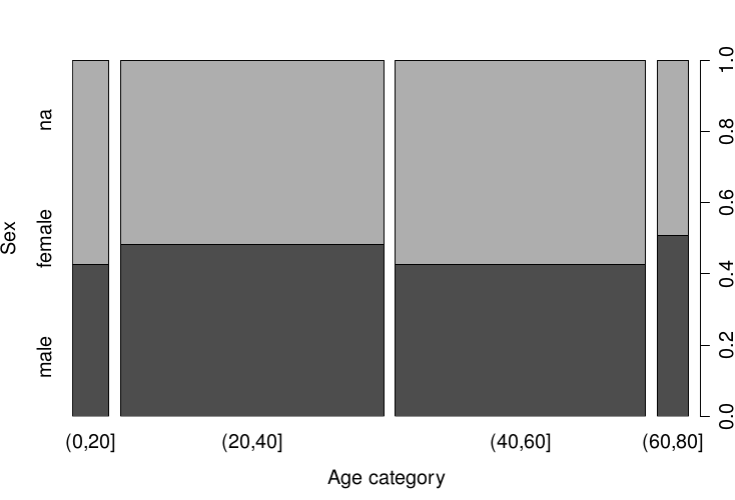
\includegraphics[width = 12cm]{age-sex-plot}
 \end{center}
 % cc-ems.pdf: 792x612 pixel, 72dpi, 27.94x21.59 cm, bb=0 0 792 612
\caption[Diagnostic plot to check the sanity of age and sex inputs.]{Diagnostic
plot to check the sanity of age and sex inputs. (Square brackets
indicate that the endpoint is not included in the set --- see
International Organization for Standardization
\href{http://www.iso.org/iso/catalogue_detail?csnumber=31887}{(ISO) 80000-2:2009},
formerly \href{http://en.wikipedia.org/wiki/Interval_(mathematics)}{ISO 31-11}
on ``mathematical signs and symbols for use in physical sciences and technology'').}
 \label{fasp}
\end{figure}
These common-sense methods of data checking may seem overly simplistic to warrant
mention. Yet such basic sanity tests are the `bread-and-butter' of
quantitative analysis. They ensure that the data are properly
understood \citep{Wickham2008}. Had the input data represented in \cref{fasp}
contained an equal proportion of people under 20 as over 20, for example,
one would know that the input data for commuters was faulty.
This approach, whereby major
problems are revealed early on in frequent tests, is preferable to waiting
until the results of the full spatial microsimulation are analysed. Hours were
saved, and understanding of the input datasets was improved.\footnote{The
use of the
same command to check model output was crucial to the identification of
important errors, including a small mistake in the code which led to large
errors in the synthetic microdata output for the distance constraint variables.}

The basic tenet of spatial microsimulation is that simulated and actual data
should match at the aggregate level \citep{Ballas2007simb}.
This knowledge led to the
continual plotting of census vs simulated results in the early stages of the
model construction, and the development of more
sophisticated plots (see \cref{fig:IPF-4c}).
Still, the humble scatter plot was used frequently for
preliminary analysis. To provide an example, after the model was run for
Yorkshire
and the Humber region for 20 iterations, I was confident the results were
correct: the results had been tested for Sheffield, and everything
\emph{seemed} to be working as expected.

Knowledge of how model-census fit should look started alarm bells
ringing when an imperfect plot was discovered:
% (largely by luck, as I was looking at the fit
% between only some of the variables, and happened to think the number of people
% taking very short trips could be subject to higher than normal levels of
% error). % What does this contribute? Nowt.
\cref{fig:error} (A) was cause for concern, not only for the low
correlation between the two variables (which was still greater than 0.8), but
because the direction of the error: the model had \emph{always} overestimated the
number of people travelling short distances to work in past runs.
This seemed suspicious, and the relationship was plotted for earlier constraints
to identify where the problem was variables were plotted.
\cref{fig:error} (B) was the
result of this, after constraining by distance.
Something had clearly gone wrong because no people who work
from home had been registered in the aggregate output. These issues led to
a re-examination of the code contained
within the file cats.r. It was found that a faulty placement of an
equals sign (such that values ``greater than or equal'' to 0 were accepted as 0
- 2 km travel to work). The problem was solved, and the model correlation
improved as a result (\cref{fig:error} (C)).

The two examples described above provided insight into how the model was
performing by its own standards. The more challenging stage is to validate
the model against factors external to it. % This is further discussed !!!

\begin{figure}[h]
  \begin{center}
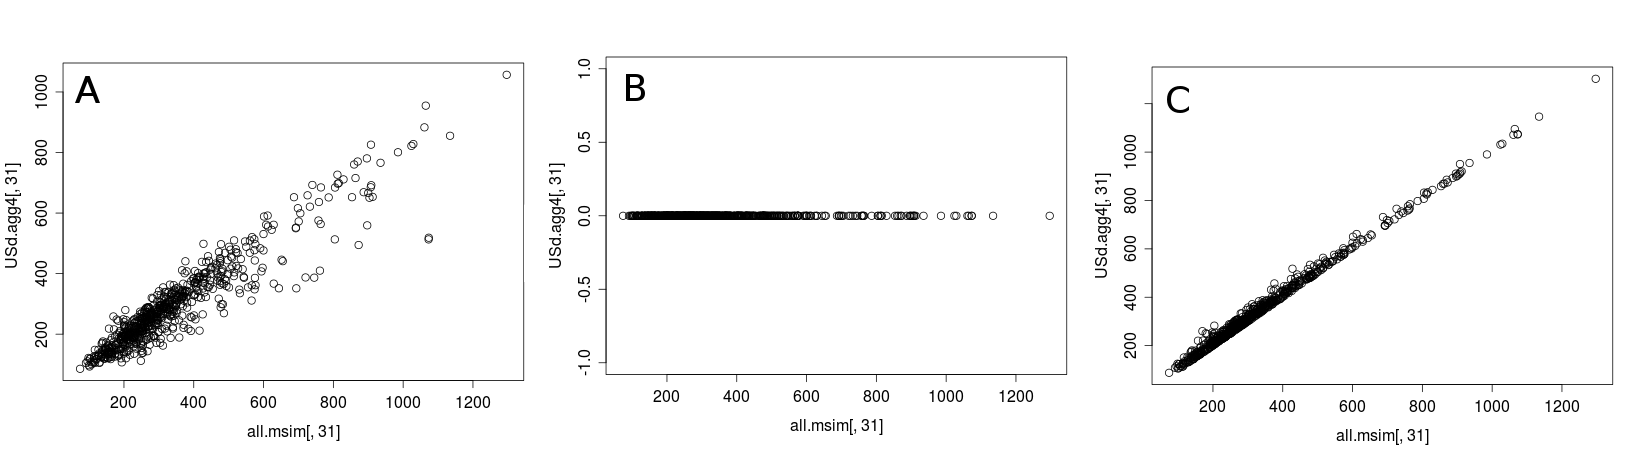
\includegraphics[width=15cm]{errors3-1}      \end{center}
 % cc-trans.png: 1113x529 pixel, 72dpi, 39.26x18.66 cm, bb=0 0 1113 529
 \caption[Diagnostic plots to identify model error]{Three diagnostic plots used
to identify a code error in the spatial microsimulation model (for the
distance category `travels 0--2 km to work'). The x-axis is
census data, the y-axis is the simulated result. A) First plot
analysed (for iteration 20); B) second plot, which illustrated the source of the
problem, in the distance constraint; C) satisfactory diagnostic plot,
after the problem had been resolved.}
 \label{fig:error}
\end{figure}

\subsection{Model validation}
\label{meval}
% {\color{red} Should this section be in a later chapter?} !!!
Beyond `typos' or simple conceptual errors in model code, more fundamental
questions should be asked of spatial microsimulation models. The validity
of the assumptions on which they are built, and the confidence one should have
in the results are important. This is especially true of models designed to inform
policies which have the potential to influence quality of life. Yet
evaluation and `validation' are
 problematic for any models that attempt to explain extensive, complex
systems such as cities or ecosystems. The urban modelling approach, of which
spatial microsimulation of commuters is a subset, has been grappling with this
problem since its infancy. Lacking a crystal ball, time-machine or settlements
on which controlled experiments can be performed, the difficulty of model evaluation can
seem intractable: ``only through time can a model be verified in any
conventional sense of the word'', by comparing the range of projected futures
with the reality of future change in hindsight \citep[p.~15]{batty1976urban}.

Why do urban models pose such a problem? Previously unknown knock-on impacts
cannot be ruled out due to the vast number of links between system
elements.\footnote{It is, of course, impossible to know how every resident of
an area interacts with every other, let alone predict the future impacts of
this interaction, even in the era of ubiquitous digital communications.
}
Rigorous real-world testing is usually impossible due to the scale of the system
and ethics involved with intervening in peoples' lives for the sake of research.
Controlled experiments cannot be performed on real settlements in the
same way that experiments can be performed in the physical sciences and, even if
two similar settlements could be found on which to apply different
interventions, there is no guarantee that all other factors will be held
constant throughout the duration of the experiment. %%% Refs!!!
% Going off on a bit of a waffle to be fair

Additional evaluation problems apply to spatial microsimulation models in
particular for a number of reasons, including:
\begin{itemize}
 \item The aggregate values of categorical `small area' constraint variables are already known from the Census, 
 so should be accurate. Checking the distribution of continuous variables such as 
 age and distance travelled to work against these crude categories is 
 problematic.\footnote{For example, if 50\% of
commuters in a particular area travel 2--5 km to work according to the Census,
does that mean that there is a normal distribution of trip distances with the
mean focussed on 3.5? Or is it more likely that there is a single large
employer located somewhere between 2 and 5 km from the bulk of houses in the
area, which accounts for the majority of these jobs and leads to a skewed
distribution of home-work distances. In every event, spatial microsimulation
will ignore such subtleties and smooth out extreme skewness by approximating the
national distance trends within each distance bin.
}
  \item Target variables are not generally known as geographic
aggregates. Therefore checking their validity for small areas is 
difficult: new surveys may be needed.
  \item Spatial microsimulation results in long lists of individuals for each
zone. With thousands of individuals in each zone and hundreds of zones, the
datasets can become large and unwieldy.
\end{itemize}

Regarding the target variables, inaccuracies can be expected because they are
determined entirely by their relationships with constraint variables. Also
it can be expected these relationships will not remain constant for all places:
perhaps in one area the number of female drivers is positively correlated to
distance travelled to work, yet there may be a different strength of
correlation, or the variables may be unrelated in another.

As mentioned above, validation of target variables is especially problematic
due to lack of data. To overcome this problem, two techniques were employed.
First, the interaction between constrained variables and unconstrained
variables was tested using data from the Census. Second, an additional dataset
from the UK's National On-line Manpower Information System
(Nomis) was harnessed to investigate the
correlation between unconstrained `interaction' variables --- those
composed of two or more constraint variables such as `female driver'.

The first approach tested the model's ability to simulate income. Although
income data are lacking for small areas, Neighbourhood Statistics
provides estimates of net and gross household incomes at the MSOA level. For the purposes of
this study, equivalised net income was used. The fit between the Neighbourhood
Statistics and simulated values are displayed in \cref{fig:income-test}.

\begin{figure}[h]
 \centering
 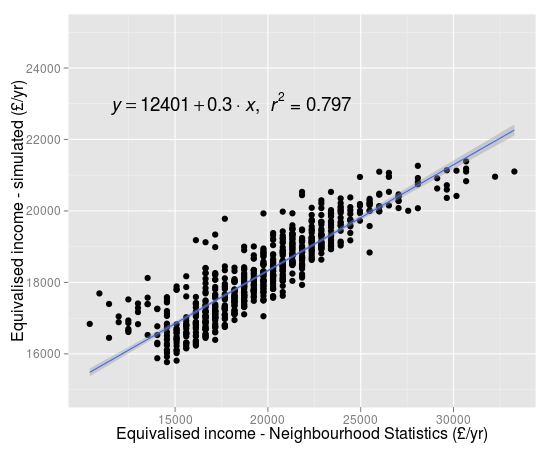
\includegraphics[width=12cm]{Income-check-morevars}
\caption[Scatter plot of simulated vs official estimated income]{Scatter plot
illustrating the correlation between mean
income simulated from the model and official estimates at the MSOA
leve.}
 \label{fig:income-test}
\end{figure}

The results show the microsimulation model could be used to predict income
(modelled income), accounting for almost 80\% of the variation in the
Neighbourhood Statistics data using an ordinary least squares (OLS) regression
model.
This is impressive, given that the aim of the model is not to simulate
income but energy costs of work travel, based on mode, distance, age/sex
and class. Of these socio-economic class is the only constraint
variable traditionally thought to be closely associated with income.
The main problem with the income estimates generated through spatial
microsimulation is the small range of estimates simulated:
the standard deviation was
\pounds1,194 and \pounds3,596 for the simulated and National Statistics data
respectively. (Note the
differences in the x and y axis scales in \cref{fig:income-test}.)
This underestimation of variance can be explained because social class,
distance and modes of transport are not sufficient to determine the true
variability in household incomes. Constraining by car ownership and tenure
variables would be likely to improve the fit.

The purpose of this fitting exercise is not so much to provide accurate income
estimates at the local level but to evaluate the
performance of the spatial microsimulation model. In terms of income, a variable
that is unconstrained in the model yet available from the survey data, the
spatial microsimulation model has worked well. The results suggest that the
values of unconstrained variables will not simply repeat the national average
for every small area, but will vary based on how their variation at the
national level is related to the constraint variables. In this case, the
assumption that the relationships between the target variable (income) and
constraint variables at the local level (in Yorkshire and the Humber) are
similar to the relationships between these variables at the national level,
receives support. How well does the model simulate other target variables such
as environmental habits, domestic energy use and levels of deprivation?
These are interesting
questions that merit further attention based on available data.

The second approach relies on Nomis, which provides cross-tabulations of census
variables, for example transport mode by class. The downside is that the data
are randomised, as stated at the bottom of each of their small-area census
tables: ``Figures have been randomly adjusted to avoid the release of
confidential data'' (this phrase appears in many of Nomis's tables.
One example can be found here:
\href{http://www.nomisweb.co.uk/livelinks/4652.xls}{http://www.nomisweb.co.uk/livelinks/4652.xls}).

In order to harness Nomis data to test the accuracy of the microsimulation
model for calculating, it was first necessary to establish how accurate Nomis
data are. How much have Nomis data been randomised, and in what way? 
This question is relatively easy to 
answer because of the census variables shared between those published 
by Nomis and by Casweb at the MSOA level. Scatter plots
suggest Nomis data are faithful to the original census results:

\begin{figure}[h]
 \centering
 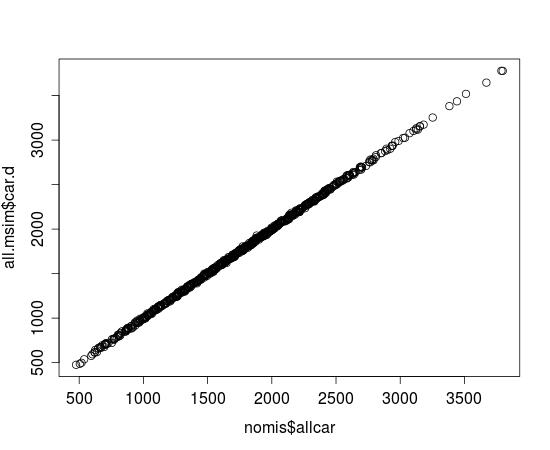
\includegraphics[width=6.6cm]{nomis-vs-cens-car}
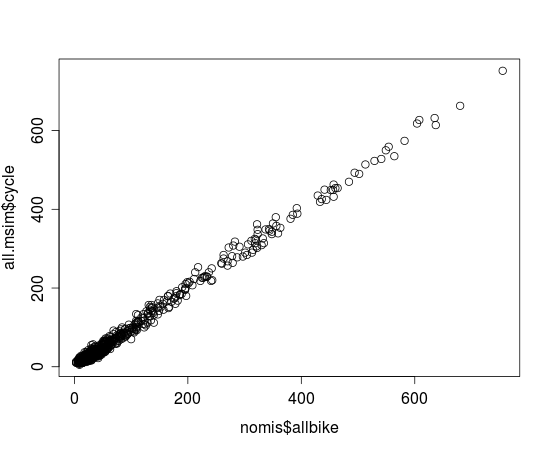
\includegraphics[width=6.6cm]{nomis-vs-cens-bike}
 % Graph-line.pdf: 516x363 pixel, 72dpi, 18.20x12.81 cm, bb=0 0 516 363
 \caption[Scatter plot of error introduced in Nomis data]{Scatter graphs
illustrating the fit between Nomis
and Casweb versions of the same census variables. The correlation (Pearson's r)
is 0.9998 and 0.9969, for the number of car drivers and number of cyclists in
each MSOA respectively.}
 \label{fig:nomis-vs-cens-car}
\end{figure}

From \cref{fig:nomis-vs-cens-car} it is interesting to note that the
correlation decreases for cyclists. This, it was inferred, could represent
an increase in the signal-to-noise ratio for variables with small values
to a fixed randomising factor.  To test this, the errors were plotted for
variables with large (car drivers) and small (cyclists) totals. The results
indicate that the noise added by randomisation is equal for each variable,
regardless of the cell count (\cref{fig:nomis-ers}).

 \begin{figure}[h]
 \centering
 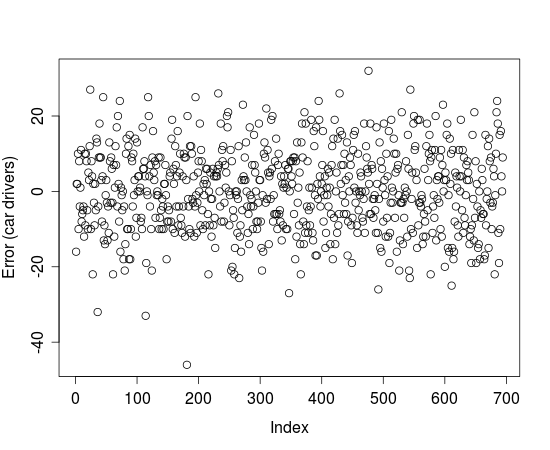
\includegraphics[width=6.6cm]{car-ers}
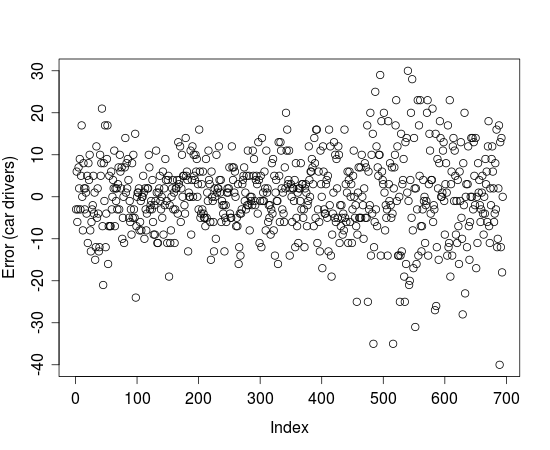
\includegraphics[width=6.6cm]{bike-ers}
 % Graph-line.pdf: 516x363 pixel, 72dpi, 18.20x12.81 cm, bb=0 0 516 363
 \caption[Errors associated with Casweb census variables]
{Errors (Casweb values -- Nomis values) associated with car driver
(right) and bicycle commuter (left) census variables.}
 \label{fig:nomis-ers}
\end{figure}

The errors seem to be similar, with a range of approximately 70 and a mean of
zero. This observation is confirmed by descriptive statistics for each set of
errors (standard deviation = 11.01, 9.47; mean = 0.15, 0.23) for car driver and
cyclist variables respectively. We can therefore conclude that the error added
by randomisation is constant for each variable and this was confirmed by plotting
the errors for additional census variables. Q-Q plots --- which compare the 
quantile values of one distribution against another, in this case those of 
the errors against those of the normal distribution --- suggest that the
distribution of error is approximately normal.

These exploratory methods provide confidence in the Nomis data, but only for
relatively large cell counts (the signal-noise ratio approaches 1:1 as the cell
count approaches 20): therefore evaluations based on Nomis data are better
suited to cross tabulated categories that have high cell counts, for example car
drivers. In our microsimulation model, both gender and mode of
transport are constrained, but not simultaneously, so the fit between the Nomis
cross-tabulation and the cross-tabulation resulting from our model provides
some indication of accuracy. The results are presented in
\cref{no-vs-sim-mcar}. Interestingly, the accuracy of this `partially
constrained' simulated target variable appears to be worse than that of the
completely unconstrained income variable (compare \cref{no-vs-sim-mcar}
and \cref{fig:income-test}). In both cases, the correlation is reasonably strong
and positive (0.47 and 0.80 respectively). However, as with the income
estimates, the \emph{distribution} of estimates arising from the model
is less dispersed than actual data: the standard deviation for the former (0.30)
is substantially less than for the latter (0.44). This illustrates the tendency
of spatial microsimulation models to underestimate the extent of spatial
variation. %%% citep{} ???

\begin{figure}
 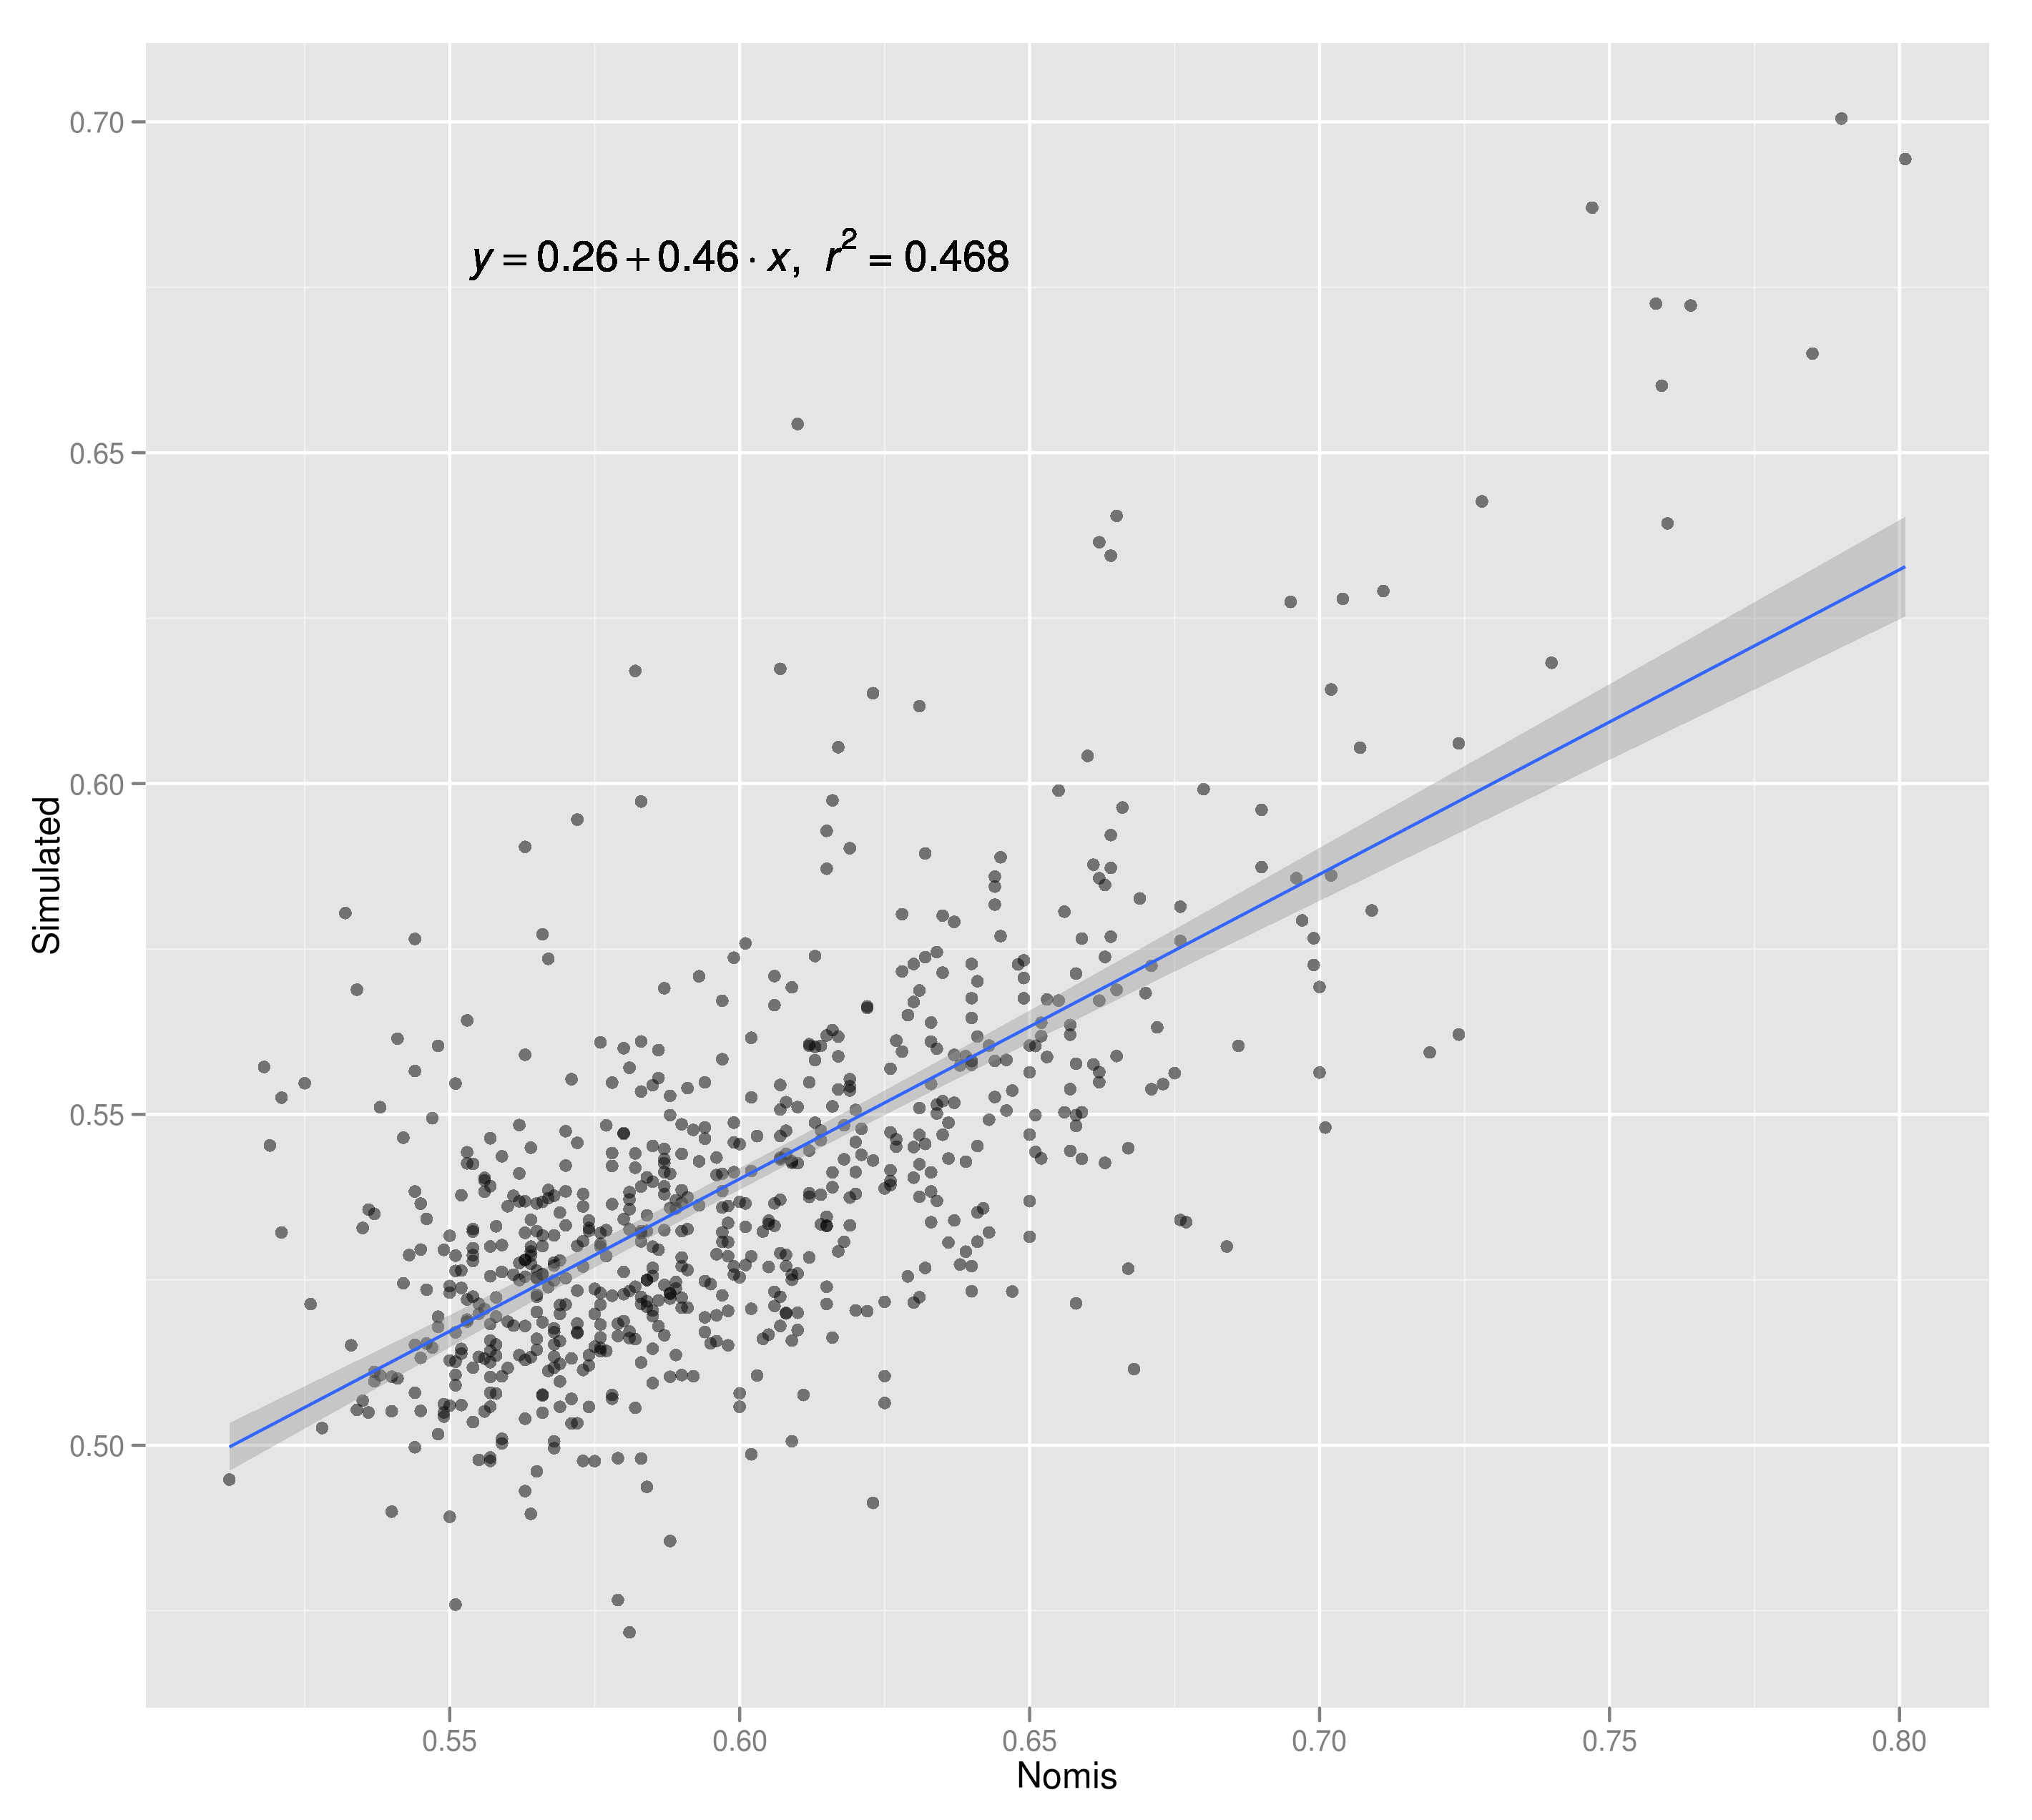
\includegraphics[width = 12 cm]{no-vs-sim-mcar}
\caption[Scatter plot of the proportion of male drivers]{Scatter plot of
the proportion of male drivers in each MSOA area in
Yorkshire and the Humber according to simulated and Nomis data.}
\label{no-vs-sim-mcar}
\end{figure}

\subsection{Additional validation methods}
The methods described above illustrate the techniques used to prevent
model errors and ensure that the results were compatible with external data
sources. But they only scratch the surface of what is possible in terms of
model validation. This section will not go into detail. Its
purpose is to draw attention to
additional methods that could be conducted as lines of future research
and discuss the merits of each. Specifically, the following additional validation
methods could (given sufficient resources) be implemented:
\begin{itemize}
 \item Primary data collection of target variables at the individual level
 in specific areas to  validate the spatial microdata locally.
 \item Comparing of the spatial microdata over entire region with a
 survey data that specifies home region of resident.
 \item Aggregating local model outputs to coarser geographical levels at which
 cross-tabulated data are available.
 \item Comparison of mode and distance data with external correlates of personal
 travel (e.g.~MOT data on distance travelled and bus usage data).
\end{itemize}

Other than the sanity check of age-sex ratios presented in \cref{fasp},
the evaluation methods considered above operate at the level of geographically
aggregated counts. However, the unique feature of spatial microsimulation is
its simulation of individuals. Evaluation techniques should therefore operate
at the individual level as well.
% The potential for evaluation of the simulated
% spatial microdata outputs is limited by the availability of official spatial
% microdata. As a result this section is short and, for the most part,
% purely theoretical.
%
% The available datasets were introduced with reference to an idealised
% `perfect' dataset on commuting \cref{fdata-ideal}. In the same way, we will
% describe methods of evaluating the microsimulation model at the individual
% level with reference to the ideal of unlimited data. This will inform the
% discussion of how best to use the individual level data that is available
% for model evaluation...
Because simulation, almost by definition, estimates something that is not
otherwise known, it is hard to find reliable individual level
data against which the estimates can be evaluated. For this reason
individual level surveys could be conducted in a specific area where
spatial microdata have been generated. To take one example, a randomised
sample of households could be taken in a single ward. Respondents would be
asked the mode of travel to work, distance and frequency of trip and
other variables. This would allow the model to be evaluated
not only in terms of the correlations that it outputs between different categories,
but also for the evaluation of the assumptions on which the energy calculations %??? where
are based.

One of the main advantages %cited where???
of spatial microsimulation over just using aggregated data is that it provides
insight into the \emph{distribution} of continuous variables within each zone,
rather than just counts of categories which are often rather coarse. T-tests and
Analysis of Variance (ANOVA) tests could then be used to check if the
mean and variance of the simulated and survey data are statistically likely
to be from the same population. However, the raw results of IPF are not
conducive to such tests at the individual level because they do not contain
whole individuals. Integerisation of the weight matrices is needed.


\section{Integerisation} \index{integerisation}
A question raised by this research is this: How do integerised IPF results
compare with other (e.g. combinatorial optimisation) approaches to spatial
microsimulation?
Studies have compared non-integer results of IPF with
alternative approaches \citep{harland2012}, but not like-with-like.

\section{Extensions to the basic model}
\label{discuss}

\section{Acknowledgements}

\label{Bibliography}
% \lhead{\emph{Bibliography}}  % Change the left side page header to
% \fancyhead[LO,RE]{\emph{Bibliography}}
\bibliographystyle{model2-names}  % Use the "unsrtnat" BibTeX style for
% \bibliography{library, lincluded}  % The references (bibliography) information are stored
\bibliography{/home/robin/Documents/Microsimulation.bib}  % The
% /nfs/foe-fs-01_users/georl/Documents/Microsimulation,

\addtocontents{toc}{\vspace{2em}}  % Add a gap in the Contents, for aesthetics

%% -----------------------------------------------------------

\printindex
\label{index}
\phantomsection
\addcontentsline{toc}{chapter}{Index}
\end{document}  % The End
